\documentclass{kththesis}

\usepackage[export]{adjustbox}
\usepackage{amsmath}
\usepackage[style=numeric,sorting=none,backend=biber]{biblatex}
\usepackage{booktabs}
\usepackage{caption}
\usepackage{color}
\usepackage{csquotes} % Recommended by biblatex
\usepackage[super]{nth}
\usepackage{float}
\usepackage{relsize}
% \usepackage{siunitx}
\newcommand{\num}[1]{{#1}}
\usepackage{soul}
\usepackage{subcaption}
\usepackage{wrapfig}

\addbibresource{references.bib} % The file containing our references, in BibTeX format
\renewcommand{\arraystretch}{1.2}
\newcommand{\source}[1]{\vspace{-5mm}\caption*{\textcolor{darkgray}{Author: {#1}}\vspace{-7mm}} }
\captionsetup[table]{skip=10pt}
\restylefloat{table}

\title{Evaluating different training techniques for a convolutional neural network that classifies Alzheimer's disease}
\alttitle{Utvärdering av olika träningstekniker för ett CNN-nätverk som klassificerar Alzheimers sjukdom}
\author{Karl Lundstig}
\email{lundsti@kth.se}
\supervisor{Jeanette Hällgren Kotaleski}
\examiner{Örjan Ekeberg}
\programme{Degree Project in Computer Science, DD142X}
\school{School of Electrical Engineering and Computer Science}
\date{\today}

% Uncomment the next line to include cover generated at https://intra.kth.se/kth-cover?l=en
\kthcover{kth-cover.pdf}


\begin{document}

% Frontmatter includes the titlepage, abstracts and table-of-contents
\frontmatter

\titlepage

\begin{abstract}
  English abstract goes here.
  $$\int \gamma$$

\end{abstract}


\begin{otherlanguage}{swedish}
  \begin{abstract}
    Träutensilierna i ett tryckeri äro ingalunda en oviktig faktor,
    för trevnadens, ordningens och ekonomiens upprätthållande, och
    dock är det icke sällan som sorgliga erfarenheter göras på grund
    af det oförstånd med hvilket kaster, formbräden och regaler
    tillverkas och försäljas Kaster som äro dåligt hopkomna och af
    otillräckligt.
  \end{abstract}
\end{otherlanguage}


\setcounter{secnumdepth}{2}
\setcounter{tocdepth}{2}
\tableofcontents


% Mainmatter is where the actual contents of the thesis goes
\mainmatter

\chapter{Introduction}

In the last couple of years machine learning and specifically deep learning have been applied successfully on several problems. These problems cover various areas, such as speech recognition, image recognition \parencite{krizhevsky2012imagenet}, and even board games \parencite{silver2018general}. One area which could benefit greatly from effective image recognition and analysis is medical diagnostics.

Alzheimer’s Disease (AD) is a neurodegenerative disease, and the leading cause of dementia. There is currently no cure, but early detection is still important as it can be beneficial to the patient~\cite{factsfigures2018}.

Many studies~\cite{islam2017novel, islam2018early} shows promising results for identifying and classifying Alzheimer’s Disease using structural MRI data. These studies are mainly performed on the OASIS~\cite{oasis} or ADNI~\cite{adni} datasets.

\section{Research Question}
This study will not try to achieve state-of-the-art results on Alzheimer's disease diagnosis; instead the goal is to evaluate the performance of a simple CNN model on medical data when using various training schemes. The model's accuracy will be measured starting from the simplest strategy, and then various improvements will be incrementally added and evaluated.

\chapter{Background}

\section{Alzheimer's Disease}

Dementia is a group of symptoms that may have many different causes. One common cause is Alzheimer's disease, a degenerative brain disease that is estimated to occur in 60\% to 80\% of dementia cases. In half of these cases of dementia Alzheimer's is the only cause, while many other also have evidence of other changes to the brain~\cite{factsfigures2018}.
Individuals with Alzheimer's disease can experience multiple symptoms, which can vary over the course of the illness~\cite{factsfigures2018}.

\subsection{Benefits of early detection}
Early (and accurate) diagnosis of Alzheimer's disease has several benefits. Those who do not have Alzheimer's but are diagnosed with mild cognitive impairment, might after testing realize that they're suffering from some other, treatable condition. There are also medical and social benefits to get an Alzheimer's diagnosis early. Neither a curing nor a slowing treatment exist, but individuals can still take some measures that helps them retain their cognitive function for as long as possible. Aerobic exercise, mental activity and social engagement may help delay cognitive decline, while medication and other intervention can help with managing symptoms. An early diagnosis can also help reduce anxiety by giving noticed symptoms a name, for both affected individuals and their family members. Finally, early diagnosis gives individuals time to make plans for the future while still having good cognitive function~\cite[p. 406-409]{factsfigures2018}.

\subsection{Brain changes}
\begin{figure}
  \centering
  \includegraphics[width=0.9\linewidth]{img/mri_scan.png}
  \caption{The three planes of a brain MRI scan.}
\end{figure}
The abnormal accumulation of two proteins (into what is called beta-amyloid plaques and tau tangles) inside the brain is one of several brain changes associated with Alzheimer's disease. These proteins interfere with neuron communication and nutrient transportation, while also triggering inflammation. Brain shrinkage, or \textit{atrophy,} eventually occurs due to cell loss. These protein changes may start as early as 20 years or more before symptoms appear~\cite{factsfigures2018}.

Brain atrophy occurs in a relatively late disease stage, when neurodegeneration has started to occur. This can be detected and measured using MRI imaging. Atrophy is a medically established predictor of an individual progressing from mild cognitive impairment to Alzheimer's disease. In addition, there seems to be a direct relationship between the severity of the atrophy and time-to-dementia. Brain atrophy is, however, not a unique sign of Alzheimer's but a measure of neural degeneration in general. Degeneration might be caused by other conditions~\cite{jack2010brain}.

\subsection{Clinical dementia rating}
Clinical dementia rating (CDR) is a score that is used to classify the stage of Alzheimer’s disease.
\begin{table}[h]
  \renewcommand{\arraystretch}{1.2}
  \begin{center}
    \caption{Clinical dementia rating}
    \label{tab:cdr_definition}
    \begin{tabular}{c|ll}
      \textbf{Score} & \textbf{Class} & \textbf{Description} \\
      \toprule
      0.0 & Non-demented & Cognitively normal. \\
      0.5 & Very mild & \hl{TODO} \\
      1.0 & Mild & \hl{TODO} \\
      2.0 & Moderate & \hl{TODO} \\
    \end{tabular}
  \end{center}
\end{table}

\hl{TODO: How is it calculated?}

\section{Artificial neural networks}
Artificial neural networks (ANNs) are computational modeling tools inspired by the neural networks found in biology. ANNs exhibit several information processing characteristics which make them useful for modeling complex real-word problems, among them non-linearity, their ability to handle imprecise information, and their ability to generalize~\cite{ANNFundamentals}. A common machine learning task is \textit{classification}. Here the machine learning algorithm is presented with a dataset containing many data points, each having some number of features and an assigned class. The goal of the machine learning model is then to learn a mapping from features to class, such that the model can be applied to new data where the class is unknown. ANNs are often used successfully for this task, but they do have the drawback that the models are opaque, or in other words they can't reason about why they give the output that they do~\cite[p. 3, 8--9]{weiss1990empirical}.

\begin{figure}
  \begin{center}
    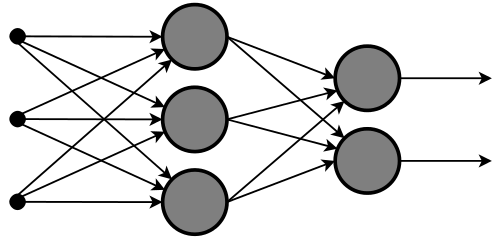
\includegraphics[width=100mm]{img/neural_network.png}
    \caption{An illustration of a multi-layer artificial neural network. }
    \source{Offnfopt / CC-BY-SA 3.0.}
    \label{fig:mlf}
  \end{center}
\end{figure}

\subsection{Structure}
Artificial neural networks can be constructed in different ways, but the most common is the so called \textit{multi-layer feed-forward neural network}, illustrated in Figure~\ref{fig:mlf}. It consists of neurons ordered into multiple layers, the first layer being the \textit{input layer} and the last one the \textit{output layer}. The layers in between are called \textit{hidden layers}. Each neuron is connected with all the neurons in the next layer, with every connection from neuron $i$ to neuron $j$ having a weight coefficient $w_{ij}$. In addition, every neuron has a threshold coefficient, or bias $b_i$. Using these coefficients and all the inputs from the previous layer, every neuron produces an output $x_i$, which can be formally written as follows:
\[x_i = \mathlarger{\varphi}\left(\sum_{j \in \Gamma^{-1}(i)}{w_{ij} \cdot x_j}\right)\]

Here $\Gamma^{-1}(i)$ is notation for the set of all neurons in the previous layer, and $\varphi$ is some \textit{activation function} which squeezes the weighted sum of all input neurons into the range $[0, 1]$, in preparation of passing the output along to the next neuron~\cite{mlfIntro}.

\subsection{Activation functions}
There are many possible choices for the activation function, but three of the most common ones can be found in Table~\ref{tab:activation_functions}. The softmax activation function is a little different than the others since it does not work on only one neuron, but instead on all neurons in the layer. In doing this, the softmax function can ensure that the sum of all the output values are equal to $1$, which is a desirable thing for the output layer when classifying into $K$ different classes. This also allows the use the \textit{cross-entropy error function} (see later section), which seems to give higher accuracy than using the sigmoid function and the \textit{least squares error function}~\cite{dunne1997pairing}.

\begin{table}[h]
  \renewcommand{\arraystretch}{1.2}
  \begin{center}
    \caption{Selection of common activation functions.}
    \label{tab:activation_functions}
    \begin{tabular}{cc}
      \textbf{Name} & \textbf{Function} $\varphi(x)$\\
      \toprule
      Sigmoid & $\displaystyle \frac{1}{1 + e^{-x}} $ \\[4mm]
      Rectifier & $\displaystyle \max(0, x)$ \\[3mm]
      Softmax & $\displaystyle \frac{e^{x_i}}{\sum_j^K{e^{x_j}}}$ \\
    \end{tabular}
  \end{center}
\end{table}

\subsection{Error functions}
To be able to train our network, we need some way to determine how `bad' a certain output is. This is done using an \textit{error function}, or \textit{loss function}. This function is averaged on the network's output on all training samples. In a classification task, the averaged loss being low means that the network is good at predicting the correct class given a certain input data. If the network performs perfectly, the error function is generally $0$. \textit{Least squares error} is a traditional error function, and if you let $x$ and $\hat{x}$ be the network's output and the wanted output respectively, the least squares error is defined as~\cite{mlfIntro}

\[ E = \sum_i{\frac{1}{2}(x_i - \hat{x}_i)^2} \] 

There is however also another error function that was mentioned earlier, the \textit{cross-entropy error} function. This has some theoretical advantages over least squares error, such as better handling when the probabilities estimated by the network is small, as well as being less dominated by large outliers. Experiments also suggest that these advantages are large enough to be useful in practice. The cross-entropy is defined as~\cite{crossentropy_squared}

\[ E = \sum_i{\hat{x}_i\left(\frac{x_i}{\hat{x}_i}\right)} \]

\subsection{Gradient descent}
\begin{wrapfigure}{r}{0.3\linewidth}
  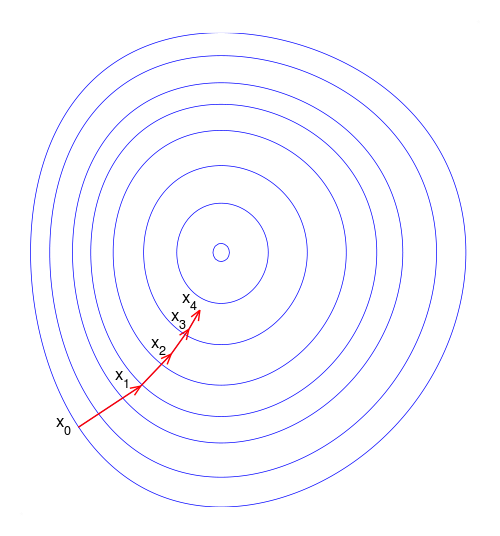
\includegraphics[width=1.6\linewidth]{img/gradient_descent.png}
  \caption{Illustration of gradient descent.}
  \label{fig:gradient_descent}
\end{wrapfigure}
To train a neural network, we want to change the weights and biases (the network's parameters) such that the error on the training set becomes as low as possible. This is done using a process called \textit{gradient descent}. Given the error function and the dataset, the neural network can be viewed a giant function, taking all the parameters as input. By finding the slope or \textit{gradient} of the parameters in the direction that decreases the error, the parameters can gradually be adjusted to find a minimum of the error function. This process is illustrated in Figure~\ref{fig:gradient_descent}. Since this gradient is calculated using the entire dataset to perform a single step, it is known as \textit{batch} gradient descent. Due to this batch gradient descent can become very slow on large datasets, and does not work at all if the dataset does not fit in memory~\cite{gradient_descent}

Because of this a variant of gradient descent named \textit{stochastic} gradient descent (SGD) is sometimes used, where the gradient is calculated using only a single training example at a time. This makes updates to the parameters much faster, but also causes the error function to jump around. This fluctuation adds noise, but also helps the model to not get stuck in local minima. SGD also has the benefit of allowing online learning, where the network can train on new data as it becomes available. In addition the overhead of calculating the gradient this many times might have a negative influence on the final performance~\cite{gradient_descent}.

There is also a third option, \textit{mini-batch} gradient descent, which aims to combine the best of both batch and stochastic gradient descent. Here the gradient calculation is performed on \textit{mini-batches} of $n$ training examples. This can help by making the updates more stable, and also helps with utilizing optimized matrix libraries that enables quickly calculating the gradient for a mini-batch. This is the method typically used when training neural networks in practice, and the term SGD is usually used to refer to this method as well~\cite{gradient_descent}.

\subsubsection{Adam optimizer}
\textit{Adam} is another, more recent method for gradient-based optimization. Its hyperparameters (parameters that adjust how the optimization method works) are intuitive and require little tuning, at the same time as Adam has high efficiency. It compares favorably to other optimization methods, and is well-suited for use in  machine learning problems~\cite{adam}.

\subsection{Learning rate}
The learning rate is a parameter that determines how large steps should be taken when performing the gradient descent. Too large a learning rate, and the network will not converge. Too small, and the convergence will take too long. A common strategy is to keep decreasing the learning rate as training progresses~\cite{Bottou2012}.

\section{Convolutional neural networks}

\subsection{Motivation}
One of the largest limitations of traditional artificial neural networks is that they struggle with the complexity of images. The input of a grayscale image of just $112 \times 112$ pixels require \num{12544} connections for every neuron in the first hidden layer. This means that the network has to have a very large number of parameters, which results in training of the network becoming very computationally demanding, as well as increasing the chances of overfitting. A model with fewer parameters to train makes overfitting less likely, which improves the network's performance~\cite{cnnIntro}.

\subsection{Structure}
Convolutional neural networks (CNNs) are specifically designed to work with images as input, and therefore has a different structure than traditional neural networks.
The neurons in a layer are not connected to the all neurons in the preceding layer, instead only connecting to a small region of it.
CNNs have three different types of layers: \textit{convolutional} layers, \textit{pooling} layers, and \textit{fully-connected} layers.
The layers are said to have three dimensions: height, width, and depth. The initial height and width correspond to the input image dimensions, while the depth represents different \textit{feature maps}.
If the images the network trains on are grayscale and has size $112 \times 112$, the input `volume' will have the dimension $(112, 112, 3)$~\cite{cnnIntro}.

\subsection{Convolutional layers}
Convolutional layers consists of a number of different \textit{filters}. These filters usually have small dimensions, say $(3, 3)$, but works on the entire depth of the input and are used to sweep, or \textit{convolve}, over the input's width and height. A $3 \times 3$ filter would have $3 \times 3 \times depth$ adjustable parameters, which forms the filter's \textit{kernel}. The output value, which will be located at the pixel in the center of the filter, is the dot product of the kernel and the current input region~\cite{cnnIntro}. For an illustration of this see Figure~\ref{fig:cnn_color_filter}.

\begin{figure}
  \begin{center}
    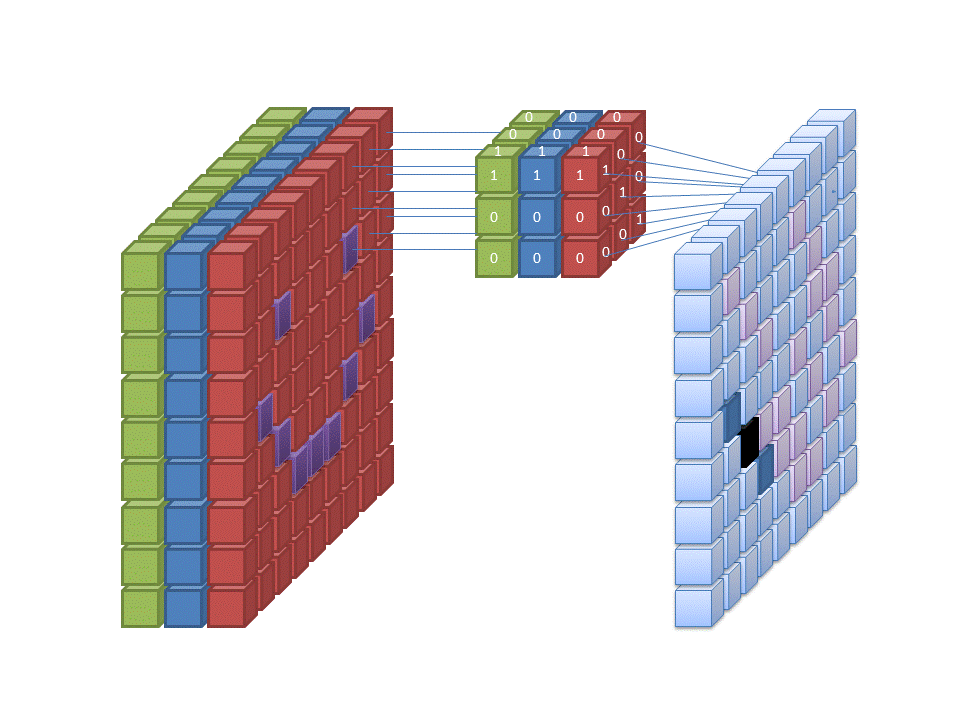
\includegraphics[width=100mm]{img/cnn_color_filter.png}
    \caption{Illustration of a filter on a color image.}
    \source{Cecbur / CC-BY-SA 4.0.}
    \label{fig:cnn_color_filter}
  \end{center}
\end{figure}

The depth of a layer's output volume in the CNN can be increased by increasing the number of filters used. The filters can pick up on different features, of which the intensity in different regions of the image will be outputted in the different depth dimensions, and picked up by later layers.

Another parameter that can be adjusted for the layer is the \textit{stride}. A stride of $1$ means that the filter is moved one step at a a time, while a higher stride of $n$ can be used to make the filter only evaluate every $n^{\text{th}}$ possible position. This reduces overlap, but has the benefit of shrinking the output volume.

For filters of size larger than $1 \times 1$, the output will have slightly smaller dimensions since the filter can't go outside the edge of the input. To avoid missing features on the edges, \textit{zero-padding} is often used. This pads the input volume with enough zeroes to make the output volume the correct size, enabling the filter to be positioned right on the edge~\cite{cnnIntro}.

\subsection{Pooling layers}
A different way of shrinking the layers' spatial dimension are \textit{pooling layers}. These are used to gradually reduce the representation's dimensionality, which reduces the total amount of parameters that need to be trained. The most common method is by using $2\times 2$ max-pooling layer. This is applied with stride 2 on the input volume, shrinking the output width and height by 2 and reducing the total output size to 25~\%. As the name implies, the output of the filter is the maximum of the input values in the region as shown in Figure~\ref{fig:max_pooling}. Pooling retains the number of depth dimensions~\cite{cnnIntro}.

\begin{figure}
  \begin{center}
    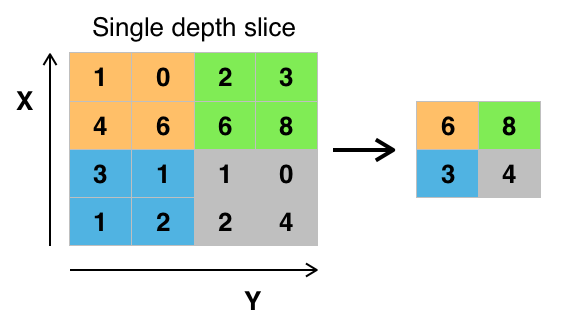
\includegraphics[width=80mm]{img/max_pooling.png}
    \caption{Example of max pooling.}
    \source{Aphex34 / CC-BY-SA 4.0.}
    \label{fig:max_pooling}
  \end{center}
\end{figure}

\subsection{Fully-connected layers}
The fully connected layers work just like they do in traditional neural networks, and are often placed at the end of a CNN network. This lets them compact all the data in the final volume into the final output of the network.

\subsection{Common architectures}
Commonly a CNN is constructed by stacking pairs of convolutional and pooling layers, before finally ending with fully-connected layers. This convolutional outputs are passed through the rectifier activation function. Another common option is to have two convolution layers before the pooling layers. This is recommended since it allows the network to learn more complicated features. The general trend in the layer volume dimensions is that they become smaller but deeper towards the end of the network~\cite{cnnIntro}. For an illustration of a typical complete CNN architecture, see Figure~\ref{fig:typical_cnn}.

\begin{figure}
  \begin{center}
    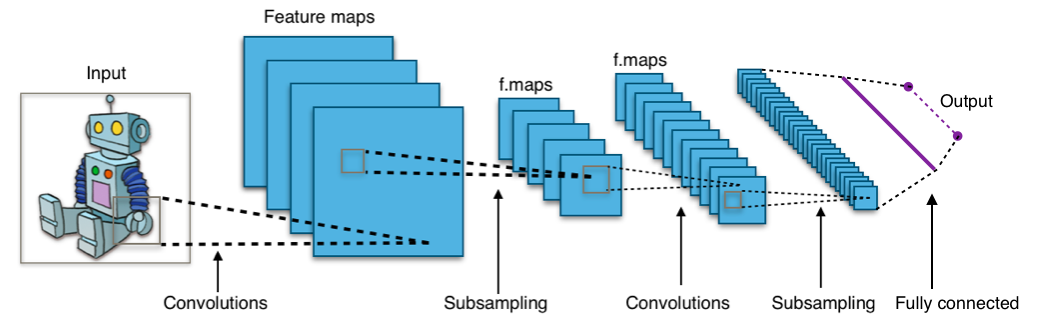
\includegraphics[width=150mm]{img/typical_cnn.png}
    \caption{Illustration of a typical CNN architecture.}
    \source{Aphex34 / CC-BY-SA 4.0.}
    \label{fig:typical_cnn}
  \end{center}
\end{figure}

\section{Evaluation of classification systems}
To evaluate a classification system an objective scoring method is needed. The most common method uses the two values \textit{precision} and \textit{recall}, together with the combined measure \textit{F1-score}. These can be calculated from the the number of true positives (TP), true negatives (TN), false positives (FP), and false negatives (FN). Descriptions of these can be found in Table~\ref{tab:tp_mm}. Precision and recall correspond to the medical terms \textit{specificity} and \textit{sensitivity}, respectively. Using these measures instead of the accuracy (the ratio of correct classifications) provides more information about what kinds of mistakes a model makes.

\begin{table}[H]
  \begin{center}
    \begin{tabular}{cc}
      \textbf{Name} & \textbf{Meaning} \\
      \toprule
      TP & Hits, number of correct identifications. \\
      TN & Number of correct rejections. \\
      FP & False alarms, number of incorrect identifications. \\
      FN & Misses, number of incorrect rejections.
    \end{tabular}
  \end{center}
  \caption{Explanation of classification results.}
  \label{tab:tp_mm}
\end{table}

\subsubsection{Precision}
In the context of classification, the fraction of guesses on a certain class that is correct is said to be the \textit{precision} of the model on this class~\cite[p.~5]{irbook}.
\[ P = \frac{\text{TP}}{\text{TP} + \text{FP}} \]

\subsubsection{Recall}
In the context of classification, the fraction of instances of class which are correctly identified is said to be the \textit{accuracy} of the model on this class~\cite[p.~5]{irbook}. This is also known as \textit{sensitivity}.
\[ R = \frac{\text{TP}}{\text{TP} + \text{FN}} \]

\subsubsection{F1-Score}
The F1-score can be used to combine the precision and recall scores into a single measure. It is defined to be the harmonic mean of precision and recall~\cite[p.~156-167]{irbook}, which can be written as
\[ F_1 = \frac{2PR}{P + R} \]

\section{Previous work}
\hl{TODO: Fill this in with more studies to compare to}
\subsubsection{Islam and Zhang}
Zhang and co.
This was done using a version of a convolutional neural network (CNN) trained on the OASIS dataset \parencite{oasis}. While their model showed acceptable performance for identifying non-demented patients, its performance on classifying demented patients was significantly worse, which could be because of the limited number of samples.

The CNN used by \textcite{islam2018early} uses a densely connected architecture that seems identical to DenseNet~\cite{huang2017densely}. DenseNet has implementations for both TensorFlow and PyTorch. A dense architecture means that each layer in the network is not just connected to the previous layer, but also to every other layer that came before it. This can speed up training and reduce overfitting by shrinking the parameter space and providing more direct connections between different parts of the network.

\chapter{Methods}
This report will evaluate three different strategies for training a convolutional neural network:
\begin{enumerate}
  \item Default training
  \item Training with equal weighting of the different classes (\textit{class-weighting})
  \item Training utilizing \textit{data augmentation}
\end{enumerate}

These methods will be trained and evaluated using the OASIS-3 neuroimaging dataset~\cite{oasis}.

The network will train for \num{1000} epochs (one epoch is one run through all training data) using each training regime, and the accuracy on the different classes will be measured. The study by Islam and Zhang resulted in a series of numerical values for accuracy, more specifically precision, recall, and f1 score. We will calculate the same values for our network trained on the larger dataset, to be able to compare our results with theirs. \hl{TODO: Compare with other studies as well.}

\section{Training methods}
\subsection{Default training}
\textit{Default training} is the least sophisticated method, and is what would be used by someone who does not put any thought into how the training should work. This is what popular machine learning frameworks will provide by default, and will provide a performance baseline. The other two methods are meant to counter the problems the default training strategy might have in our use case.

\subsection{Class-weighting}
Like the original OASIS, OASIS-3 contains many times more images of patients without or with mild ALzheimer's disease as with more severe cases (see Section~\ref{dataset}). In the study by~\textcite{islam2017novel}, they tried to correct this by weighing each class equally in the error function, no matter how large part of the dataset each class actually represents. This will be the second training method tested, to see if this behaves as expectedly and improves the performance on the rarer classes.

\subsection{Data augmentation}
When the size of the dataset is not too large, there is a risk of overfitting. Overfitting is when the network `memorizes' the data used in the training set. This causes it to have very high performance and low error on the training data, while not being able to perform well in general which will be visible when testing on the validation data. One way to battle this is data augmentation, where the dataset is in some way extended. For this test the images will be mirrored along the along the sagittal axis (right side of the brain will become the left), as well as zooming the image in or out a random value less than 20~\%. This will in effect produce an infinite training data set (albeit quite similar), in theory making overfitting less likely.

\section{OASIS-3 dataset} \label{dataset}
OASIS-3 is a longitudinal neuroimaging dataset, with data collected over the course of 30 years from 1098 adult participants from multiple studies. Of these participants 809 were cognitively normal, while 489 were at various stages of cognitive decline. Accompanying the neural imaging is (among other things) clinical assessments of cognitive function~\cite{oasis3}. I will use the T1-weighted brain scans and mental assessments which were done using the CDR system. The dataset in total contains 3393 T1-weighted MRI images and 4089 different CDR evaluations.

The subset of the dataset that will be used contains 2782 images (see skipped images in Section~\ref{image_extraction}). Of these images 20~\% were selected to be used as validation data, while the other 80~\% will be used to train the network. Since the network has never seen the validation data during training, it can be used to evaluate its expected performance on unknown MRI images. Just as in the paper by \textcite{islam2018early} I will use the CDR scores to divide the images into four classes: \textit{non-demented}, \textit{very mild dementia}, \textit{mild dementia}, and \textit{moderate dementia}. These classes are not equally represented in the dataset, with the more serious dementia cases being much less frequent. The total count of each case is shown in Table~\ref{tab:dataset_contents}, with the count in training and verification broken out.

\section{Labeling}
I will use the assessment of the subjects' CDR score to label every MRI image with the stage of dementia. However, since OASIS-3 is a longitudinal study, the MRI scans and the clinical assessments were not performed at the same time. In fact, the time between MRI scans and the closest CDR assessment can be relatively large ($\mu=116$, $\sigma=107$). The distribution is shown in Figure~\ref{fig:mri_cdr_offset}. For most of the data the time from an MRI scan to the closest CDR assessment is less than 200 days, while for some images the delay can be several hundred days.

To try to get reasonable CDR labels even when the time differences are large, a linear interpolation of the two closest CDR assessments considering the time of the MRI scan will be used when this is possible. If the MRI scan was done either before or after all of this subject's CDR assessments, the MRI scan will be tagged with the closest one.

This CDR calculation can be written as follows:
\begin{flalign*}
  \begin{aligned}
    \text{cdr} &=
    \begin{cases}
      \text{cdr}_{\text{next}}   & \text{if before all assessments} \\
      \text{cdr}_{\text{prev}} & \text{if after all assessments} \\
      \text{cdr}_{\text{prev}} + x * (\text{cdr}_{\text{next}} - \text{cdr}_{\text{prev}}) & \text{otherwise} \\
    \end{cases} & \\[5pt]
    \text{where }x &= \frac{\text{day}_{\text{MRI}} - \text{day}_\text{prev}}{\text{day}_{\text{prev}} - \text{day}_{\text{next}}}&
  \end{aligned}
\end{flalign*}

Here $0 \leq x \leq 1$ is the interpolation factor between the two assessments closest to $\text{day}_{\text{MRI}}$, the day the MRI scan was done.

\begin{figure}
  \begin{center}
    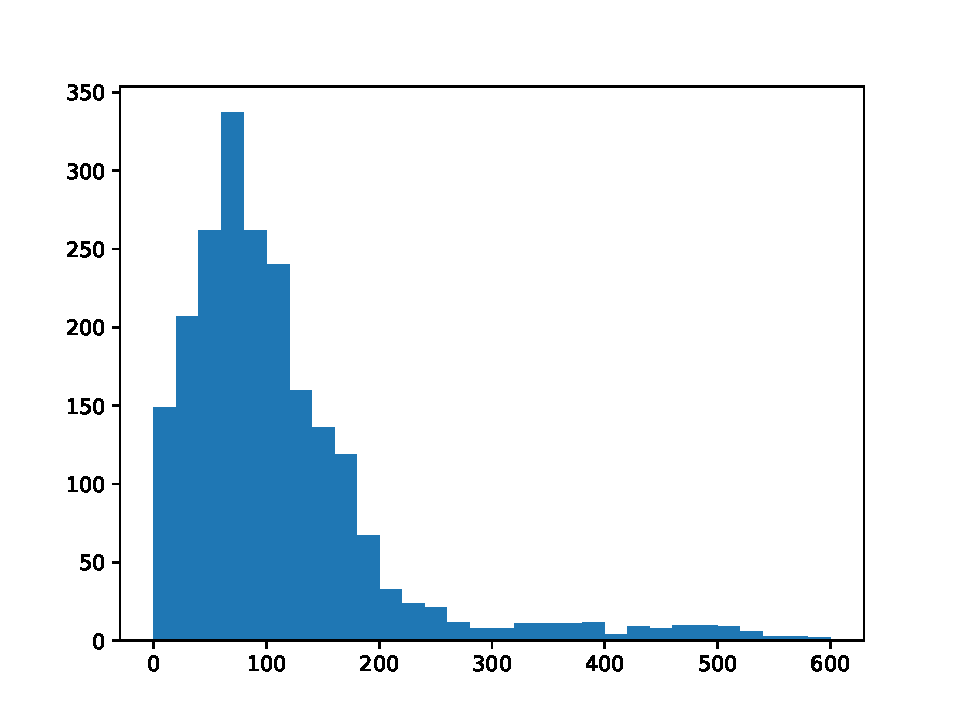
\includegraphics[width=100mm]{img/mri_cdr_offset.pdf}
    \caption{Histogram of time between MRI scans and the closest CDR assessment (in days).}
    \label{fig:mri_cdr_offset}
  \end{center}
\end{figure}

\section{Image extraction} \label{image_extraction}
During the preprocessing step the three image planes are extracted from each MRI scan. For simplicity the planes chosen are the middle one for each axis, and the raw intensity values from each scan are flattened into the normal black/white range of PNG images.

Some MRI scans are rotated the wrong way, even after trying to orient them correctly using the metadata from the scan. These images are not corrected but instead skipped.

\section{Dataset contents}

\section{Hyperparameters}
\hl{TODO: Learning rate, decay etc}

\begin{table}[h]
  \begin{center}
    \caption{Count of images belonging to each class in the dataset.\label{tab:dataset_contents}}
    \begin{tabular}{r|cccc}
      \textbf{CDR Class} & \textbf{Total} & \textbf{Training set} & \textbf{Validation set} \\
      \toprule
      Non-demented (0.0) & 2162 & 1722 & 440 \\
      Very mild (0.5) & 442 & 362 & 80 \\
      Mild (1.0) & 152 & 121 & 31 \\
      Moderate (2.0) & 22 & 17 & 5 \\
      \bottomrule
      \textbf{Sum} & 2778 & 2222 & 556 \\
    \end{tabular}
  \end{center}
\end{table}

\begin{minipage}{.7\linewidth}
  \section{Network structure}
  The network this study is going to evaluate is mostly based on the basic CNN design suggested by \textcite{cnnIntro}, with double convolutional layers joined by pooling layers. The first two layers are taken from \textcite{islam2018early}, and consists of a convolutional layer with filters of size $7 \times 7$ and stride 2, followed by a pooling layer. All the other convolutional layers use filters of size $3 \times 3$. At the end of the network there are 128 fully connected neurons which finally connect into the four output neurons. Each output neuron represents the probability of each class. The densely connected layer also uses rectified linear activation, while the output layer uses softmax activation. The network is trained using the Adam optimizer, which is a variant of SGD, and the cross-entropy loss function.

\end{minipage}
\begin{minipage}{.3\linewidth}
  \centering
  \vspace*{-20mm}
  \hspace*{0mm}
  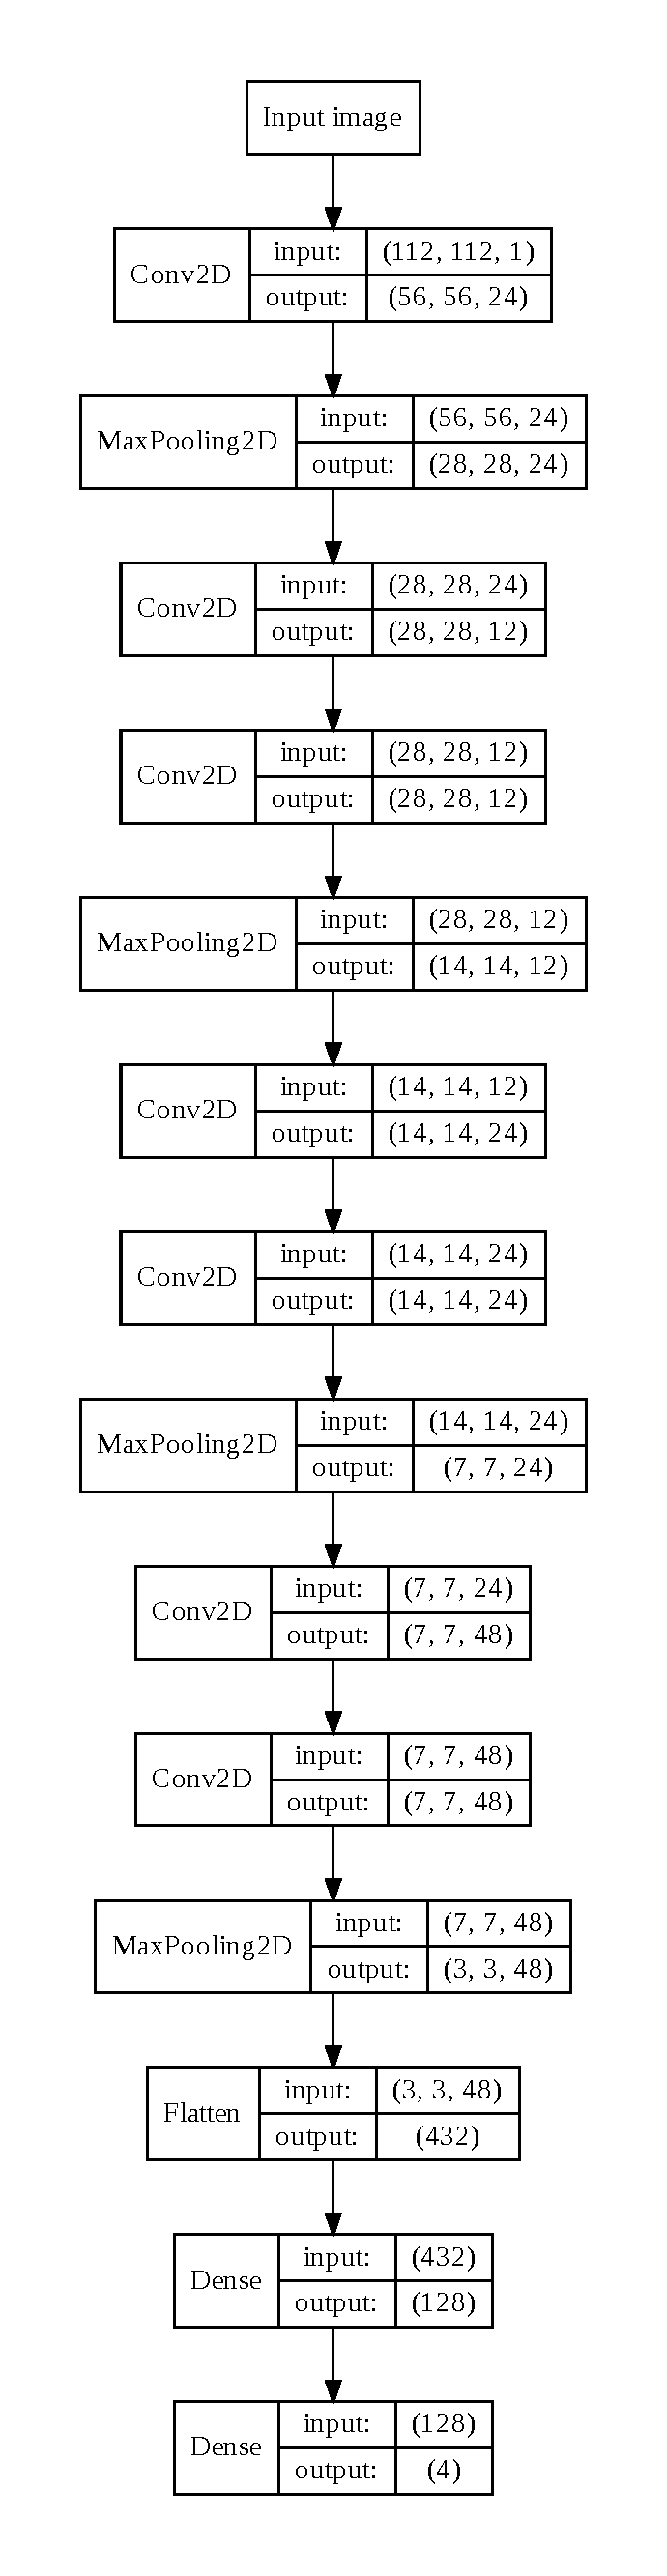
\includegraphics[width=1.8\textwidth]{img/model.pdf}
\end{minipage}

\chapter{Results}

The learning rate of the Adam optimizer was found to be very important for good results. The default learning rate of $0.001$ appears to be to large, and resulted in the network not improving. A lower rate of $10^{-5}$ resulted in better and quicker results during training.

\section{Default training}

\begin{figure}
  \centering
  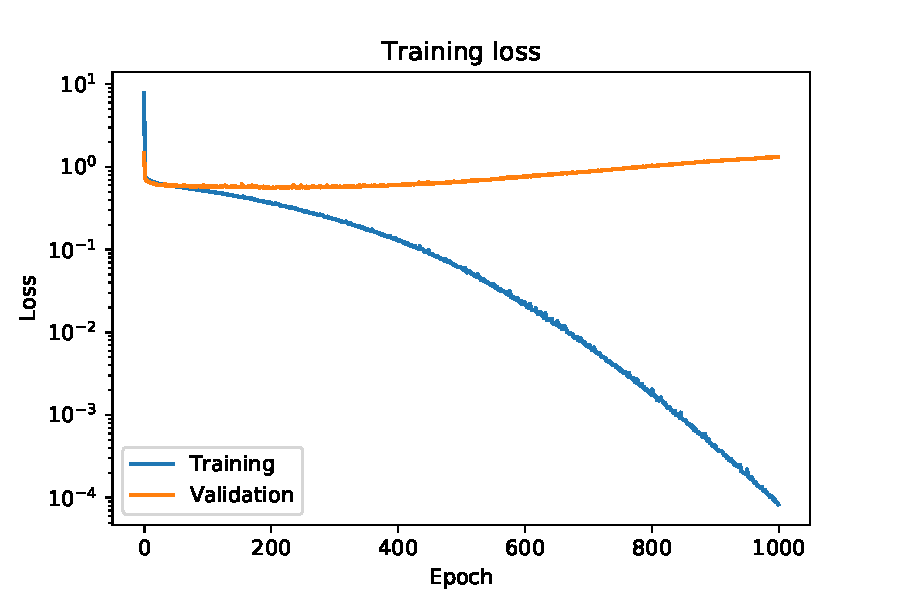
\includegraphics[width=0.9\linewidth]{img/loss_default.pdf}
  \label{fig:loss_default}
  \caption{Loss during training with the default training scheme.}
\end{figure}
\begin{figure}
  \centering
  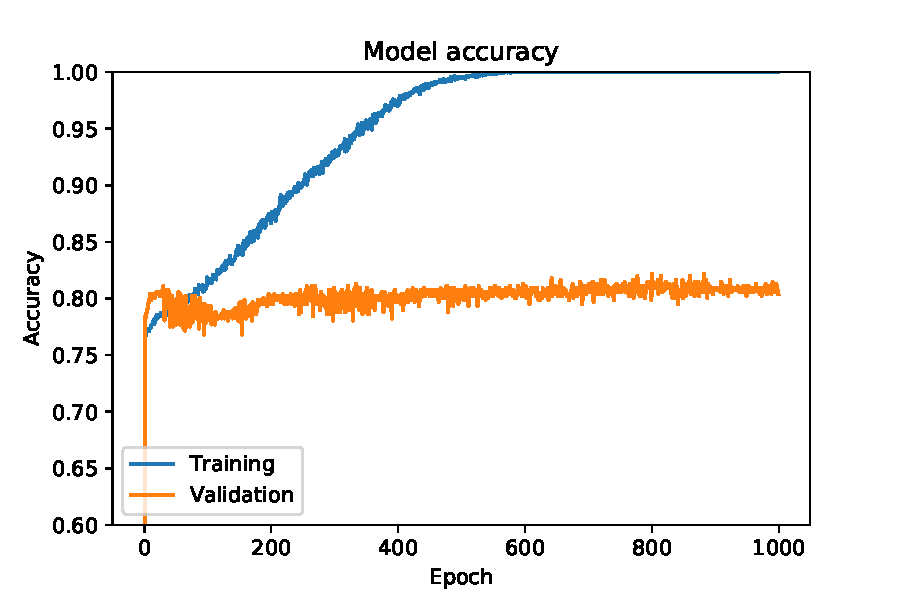
\includegraphics[width=0.9\linewidth]{img/accuracy_default.pdf}
  \label{fig:accuracy_default}
  \caption{Accuracy during training with the default training scheme.}
\end{figure}

\begin{table}[H]
  \begin{center}
    \caption{Results for default training. \label{tab:results_class_weighted}}
    \begin{tabular}{r|ccc|c}
      \textbf{CDR Class} & \textbf{Precision} & \textbf{Recall} & \textbf{f1-Score} & \textbf{Support} \\
      \toprule
      Non-demented (0.0) & 0.88 & 0.91 & 0.89 & 440 \\
      Very mild (0.5)    & 0.51 & 0.46 & 0.49 & 80  \\
      Mild (1.0)         & 0.40 & 0.32 & 0.36 & 31  \\
      Moderate (2.0)     & 0.33 & 0.20 & 0.25 & 5   \\
    \end{tabular}
  \end{center}
\end{table}
\begin{figure}
  \centering
  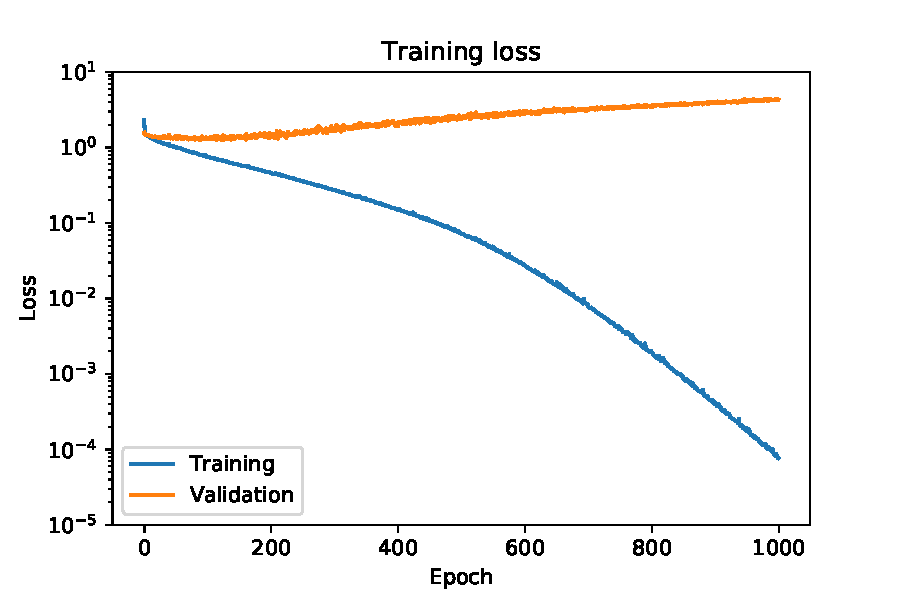
\includegraphics[width=0.9\linewidth]{img/loss_class_weighted.pdf}
  \caption{Loss during training with class-weighting.}
  \label{fig:loss_default}
  \vspace{-30mm}
\end{figure}
\begin{figure}
  \centering
  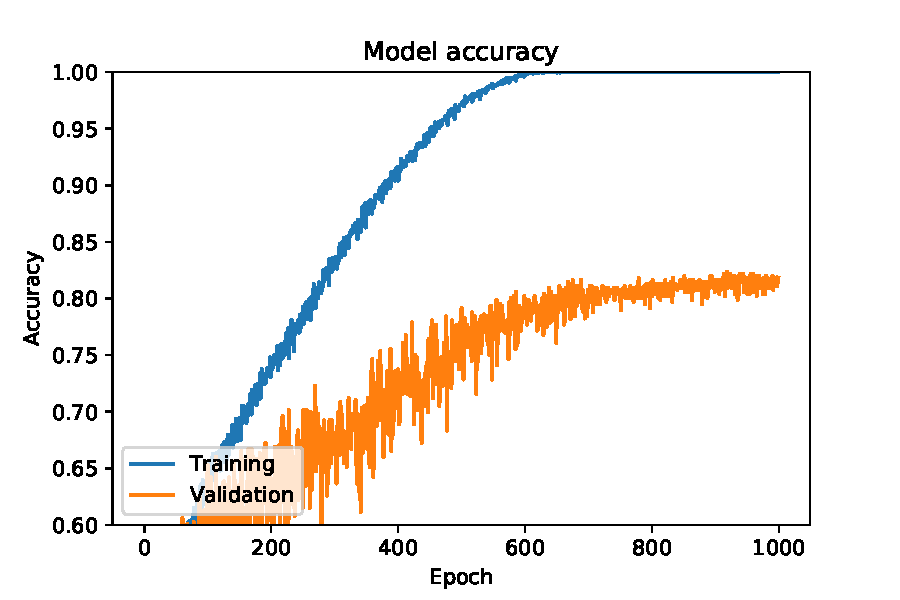
\includegraphics[width=0.9\linewidth]{img/accuracy_class_weighted.pdf}
  \label{fig:accuracy_default}
  \caption{Accuracy during training with class-weighting.}
\end{figure}

\section{Class-weighted training}
\begin{table}[H]
  \begin{center}
    \caption{Results for class-weighted training. \label{tab:results_class_weighted}}
    \begin{tabular}{r|ccc|c}
      \textbf{CDR Class} & \textbf{Precision} & \textbf{Recall} & \textbf{f1-Score} & \textbf{Support} \\
      \toprule
      Non-demented (0.0) & 0.87 & 0.93 & 0.90 & 440 \\
      Very mild (0.5)    & 0.52 & 0.41 & 0.46 & 80  \\
      Mild (1.0)         & 0.43 & 0.29 & 0.35 & 31  \\
      Moderate (2.0)     & 1.00 & 0.60 & 0.75 & 5   \\
    \end{tabular}
  \end{center}
\end{table}


\section{Training with data augmentation}
\begin{table}[H]
  \begin{center}
    \caption{Results with data augmentation. \label{tab:results_data_augmentation}}
    \begin{tabular}{r|ccc|c}
      \textbf{CDR Class} & \textbf{Precision} & \textbf{Recall} & \textbf{f1-Score} & \textbf{Support} \\
      \toprule
           Non-demented (0.0) &  0.91   &  0.77  &   0.83   &   440 \\
           Very mild (0.5)    &  0.33   &  0.57  &   0.42   &    80 \\
           Mild (1.0)         &  0.40   &  0.55  &   0.46   &    31 \\
           Moderate (2.0)     &  0.67   &  0.40  &   0.50   &     5 \\
    \end{tabular}
  \end{center}
\end{table}

\begin{figure}
  \centering
  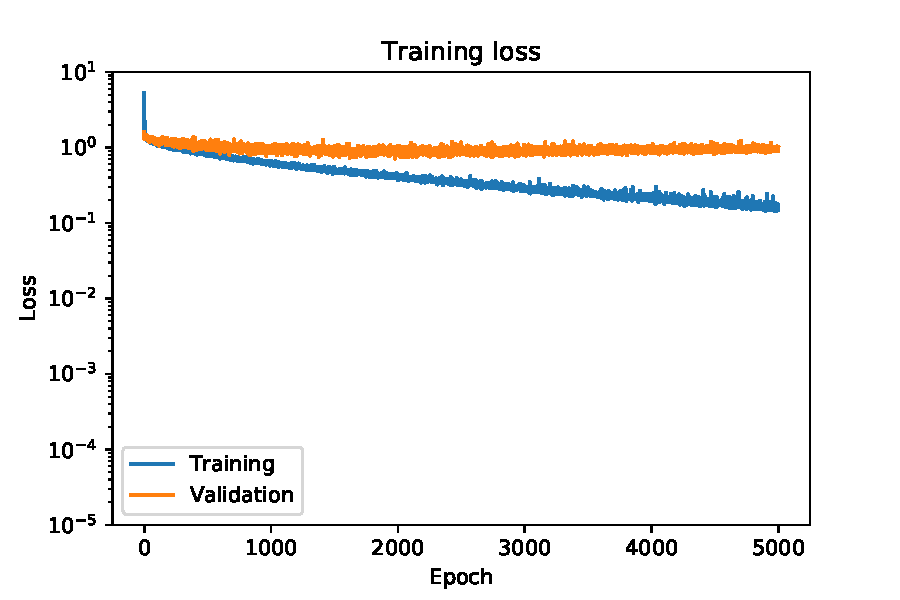
\includegraphics[width=0.9\linewidth]{img/loss_data_augmentation.pdf}
  \caption{Loss during training with data augmentation.}
  \label{fig:loss_default}
\end{figure}
\begin{figure}
  \centering
  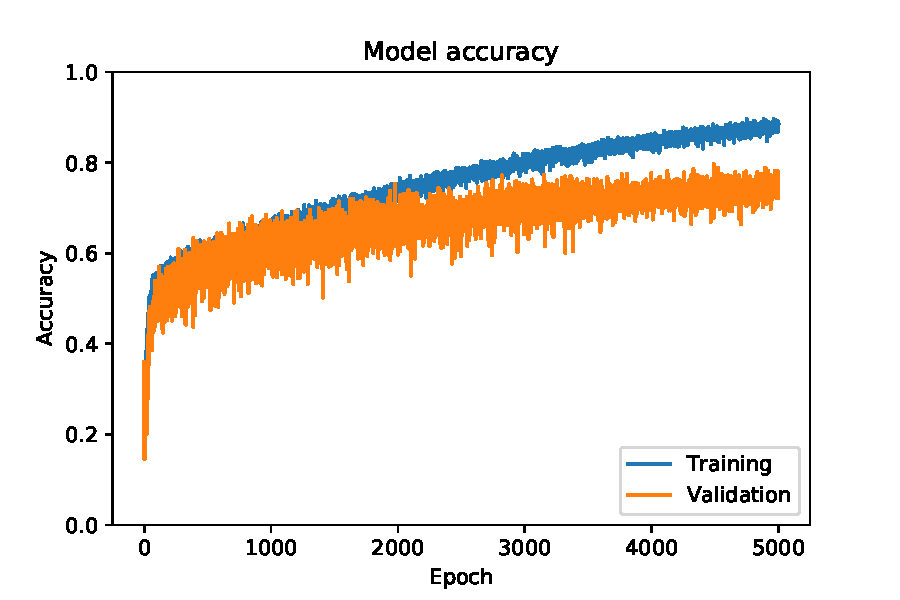
\includegraphics[width=0.9\linewidth]{img/accuracy_data_augmentation.pdf}
  \label{fig:accuracy_default}
  \caption{Accuracy during training with data augmentation.}
\end{figure}

\section{Summary of training results}
\begin{figure}[H]
  \centering
  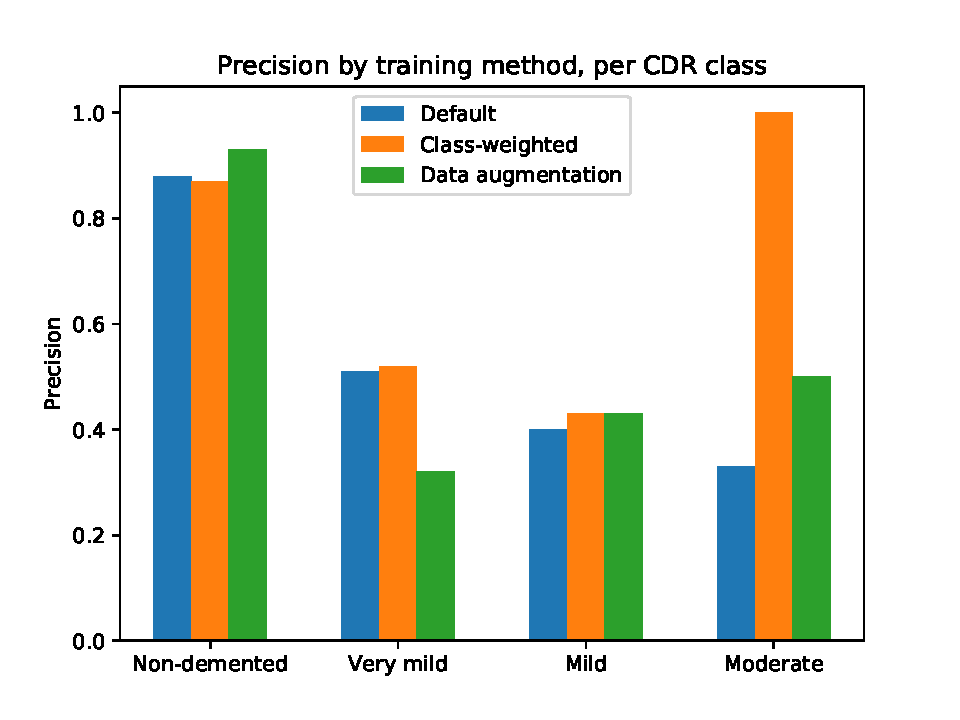
\includegraphics[width=0.8\linewidth]{img/precision_comparison.pdf}
  \label{fig:precision_comparison}
  \caption{Comparison of the precision resulting from the different training methods.}
\end{figure}
\begin{figure}[H]
  \centering
  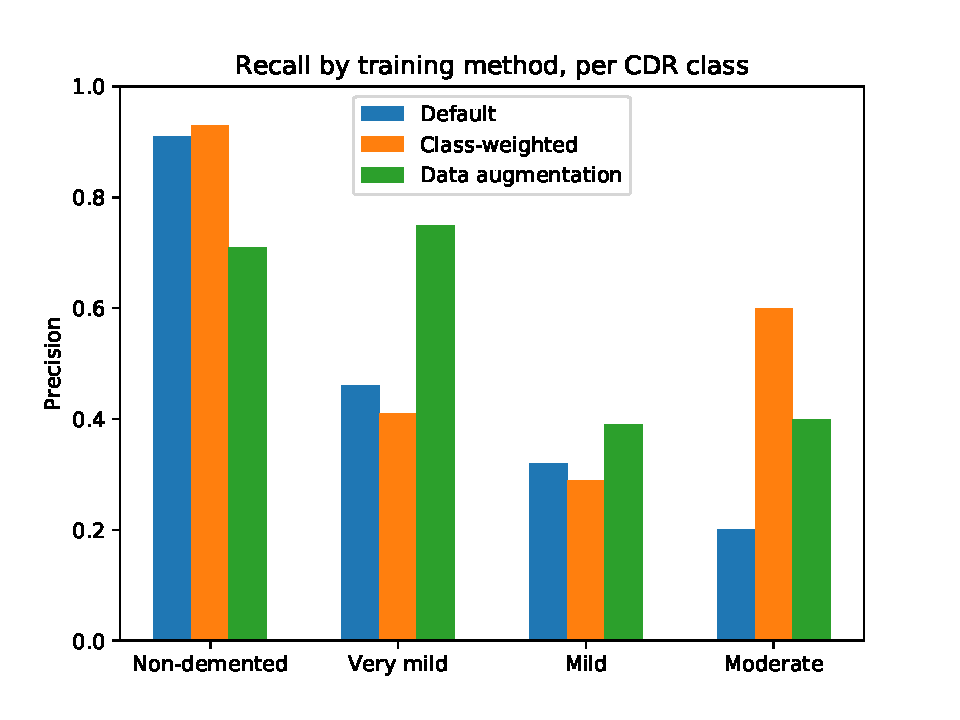
\includegraphics[width=0.8\linewidth]{img/recall_comparison.pdf}
  \label{fig:recall_comparison}
  \caption{Comparison of the recall resulting from the different training methods.}
\end{figure}

\chapter{Discussion}
Just as in the study by \textcite{islam2018early}, the low frequency of samples in the dataset showing progressed dementia is an issue. Thanks to OASIS-3 containing many times the number of MRI images as the original OASIS does, this is not too large of a problem during training, The low frequency is however very noticeable during validation, when it results in single-digit counts of the rarest class (\textit{moderate dementia}). This gives very rough knowledge of how accurate the model actually is on this type of data. It might be useful to increase the ratio of validation to training data, and in the long term create new and larger datasets that enables researchers to evaluate their models' performance with more confidence. On the other hand, detecting these progressed cases of dementia might no be very useful in practice, since by then the symptoms will be so pronounced that the diagnosis can not be missed.

\section{Method}
It is debatable exactly what good performance is in the area of computed-aided medical diagnostics. Is it more important that the model does not miss any cases (minimize false negatives), or that the model does cause any false alarms (minimize false positives)? This is not obvious, but most likely the model should prioritize finding all cases of disease. If some false positives also occur that is fine, as long as the rate is low enough for the model to be useful.

\section{Results}
\subsection{Default training}
When training without weighting the classes differently, the network starts out with an accuracy of just below 80~\%. The training data mostly contains images of cognitively normal brains, at a rate of $\frac{1724}{2162} \approx 79.7~\%$. This suggests that the network quickly learns to classify everything as this class, for a large and quick gain in accuracy which will just as quickly decrease the loss. Inspection of the output reveals that yes, this is actually the case the first few epochs. However, after training some more the network begins to try and also classify the other classes, managing a precision ranging from 30~\% to 50~\% on the three demented classifications. The accuracy steadily decreases as the classes get rarer, most likely because the loss function does not encourage exploration in order to get better on them. Since all input samples are weighted equally in the eyes of the loss function, performance on the ca.\ 20 images showing moderate dementia is worth 100 times less than the performance on the ca.\ \num{2000} images showing no dementia. If getting better on the rare classes means getting slightly worse on the dominating one, it won't happen.

\subsection{Class-weighted training}
Weighting each class equally was very important for the most rare class, \textit{Moderate}. The precision on this group increased from $0.33$ to $1.0$, and the recall from $0.20$ to $0.60$. This happened at the same time as the performance on the other classes remained on a similar level. On the classes \textit{Very mild} and \textit{Mild} precision improved slightly at the same time as recall became slightly worse, while the opposite happened on the \textit{Non-demented} class. These changes were however very small, and not significant. In conclusion, class-weighting was important for the very rare class, but not as much for the moderately rare.

If the dataset contains any rare classes, like OASIS-3 does, making sure to not disfavor them could be very important. These rare classes might be obvious, as they are here, but might also be hidden. For example, if a dataset mostly contains data collected from male subjects, a model could be biased during training and perform less well on female data, and vice versa. In cases like this 
class-weighted training could be essential for fair healthcare.

\subsection{Training with data augmentation}
Why is this so disappointing? Bug or result

\section{Future work}
\hl{TODO: Write about the limitations of this study and future work.}

\chapter{Conclusions}
A convolutional neural network was found to be a powerful model for diagnosis of Alzheimer’s disease using MRI images. Even though this study's model was not very advanced, it still achieved decent performance on a problem that is very difficult for non-trained humans.

The way the model was trained was found to be a very important factor of the network's performance. It was found to be especially important 

\chapter{Acknowledgments}
Data were provided by OASIS-3: Principal Investigators: T. Benzinger, D. Marcus, J. Morris; NIH P50AG00561, P30NS09857781, P01AG026276, P01AG003991, R01AG043434, UL1TR000448, R01EB009352. AV-45 doses were provided by Avid Radiopharmaceuticals, a wholly owned subsidiary of Eli Lilly.

% Print the bibliography (and make it appear in the table of contents)
\printbibliography[heading=bibintoc]

\appendix


% Tailmatter inserts the back cover page (if enabled)
\tailmatter

\end{document}
